\documentclass[tikz,10pt]{standalone}

\definecolor{NewHex}{HTML}{648FFF}

\begin{document}
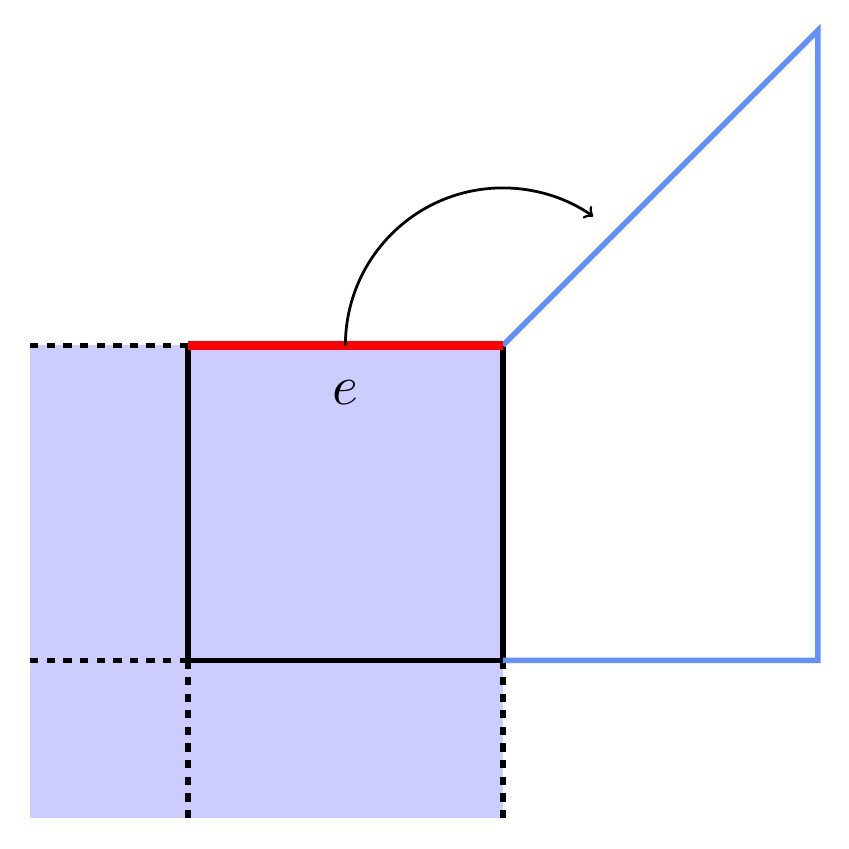
\begin{tikzpicture}[scale=4]

 %%%%%%%%%% Points pour travailler %%%%%%%%%%
 \coordinate (0) at (0,0);
 \coordinate (1) at (1,0);
 \coordinate (2) at (2,0);
 \coordinate (3) at (0,1);
 \coordinate (4) at (1,1);
 \coordinate (5) at (2,1);
 \coordinate (6) at (1,2);
 \coordinate (7) at (2,2);
 \coordinate (8) at (0,-0.5);
 \coordinate (9) at (1,-0.5);
 \coordinate (10) at (-0.5,0);
 \coordinate (11) at (-0.5,1);
 \coordinate (12) at (-0.5,-0.5);

  % Background
 \filldraw[fill=blue!20!white, draw=blue!20!white] (12) -- (9) -- (4) -- (11) -- (12) ;

 % Quads of the current layer
 \draw[color=black, line width=2] (3) -- (0) -- (1) -- (4) ;
 \draw[dashed, color=black, line width=2] (3) -- (11) ;
 \draw[dashed, color=black, line width=2] (0) -- (10) ;
 \draw[dashed, color=black, line width=2] (1) -- (9) ;
 \draw[dashed, color=black, line width=2] (0) -- (8) ;

  % New quads
  %\draw[color=NewHex, line width=2] (4) -- (6) -- (7) -- (6) -- (4) ;
  \draw[color=NewHex, line width=2] (1) -- (2) -- (7) -- (4) ;

  % Edge
  \draw[color=red, line width=3] (3) -- (4) ;
  \draw (0.5,0.85) node[color=black, scale=2] (edge) {$e$} ;
  \draw[->, line width=1] (0.5,1) arc (180:55:0.5cm);

\end{tikzpicture}
\end{document}